%%%%%%%%%%%%%%%%%%%%%%%%%%%
%                         %
%       2016.11.16.       %
%      Szakdolgozat       %
%    Tamás     LATEX      %
%%%%%%%%%%%%%%%%%%%%%%%%%%%
\documentclass[oneside,titlepage,12pt,a4paper]{report}
%\documentclass[12pt]{report}
\usepackage[centertags]{amsmath}
\usepackage{amsfonts}
\usepackage{amsthm}
\usepackage{newlfont}
%\usepackage[ansinew]{inputenc}
\usepackage[magyar]{babel}	
\usepackage[utf8]{inputenc}		
\usepackage{t1enc}				
\usepackage{graphicx}
\usepackage{color}
%\usepackage[colorlinks]{hyperref}
%\usepackage[active,new,noold,marker]{xrcs}
\usepackage{euler}
\usepackage{amssymb,latexsym}
\usepackage{amsmath}
\usepackage{graphics}
\usepackage{algorithm} 
%\usepackage{algpseudocode} %ezzel összeakadhat \usepackage{algorithmic} 
\usepackage{rotating}
\usepackage{bigstrut}
\usepackage{subfigure}
\usepackage{appendix}
\usepackage{setspace}


\newtheorem{theorem}{Theorem}
\newtheorem{corollary}{Corollary}
\newtheorem{lemma}{Lemma}
\newtheorem{proposition}{Proposition}
\newtheorem{definition}{Definition}
\newtheorem{notation}{Notation}

\textwidth=6.truein \textheight=9.truein \hoffset=-.5truein
\voffset=-.8truein

\frenchspacing				
\setlength{\parskip}{\smallskipamount}	
\renewcommand{\appendixtocname}{Függelék}
\renewcommand{\appendixpagename}{Függelék}
\DeclareMathOperator{\grad}{grad}
\DeclareMathOperator{\sgn}{sign}
\DeclareMathOperator{\PRD}{PRD}
\DeclareMathOperator{\CR}{CR}
\newcommand{\conj}[1]{\overline{#1}}

\begin{document}
\begin{titlepage}
	\parbox[t]{5.5cm}{\vspace{1cm}}
\begin{center}
	\large
	\textsc{Eötvös Loránd Tudományegyetem \linebreak Informatikai Kar} \\[2cm]
\end{center}

\begin{center}
	% Title
	\LARGE EKG jelek feldolgozása Hermite-függvények segítségével\\[0.55cm]
	\large BSc Szakdolgozat \\[1.9cm]
\end{center}

\begin{center}
	\parbox[t]{25mm}{Készítette:}
	\parbox[t]{5.5cm}
		{Dózsa Tamás\\
		ELTE IK\\
		Programtervező informatikus \\
		BSc
		}
	\\[0.9cm]
	
  \parbox[t]{25mm}{Témavezető:}
	\parbox[t]{5.5cm}{
		Dr. Kovács Péter\\
		Adjunktus\\
		ELTE IK\\
		Numerikus Analízis Tanszék
		}
	\\[4cm]
\end{center}

\begin{center}
	
\includegraphics[scale=0.7]{./Abrak/Egyeb/elte_logo.jpg}\\[1cm]
	Budapest, 2016.11.16.
\end{center}
\end{titlepage}

\tableofcontents

%%%%%%%%%%%%%%%%%%%%%
% BEVEZETES
%%%%%%%%%%%%%%%%%%%%%

\chapter{Bevezetés}
\label{intro}

\section{A modell ismertetése}
A modern orvostudományban nagy jelentőséggel bírnak 
a valamely élő szervezet által kibocsátott úgynevezett $biológiai jelek$. Ezek k\"oz\'e sorolható az $Elektro$ $Kardio$ $Gram$, vagy $EKG$,
amely a szív állapotáról képes információt adni. B\'ar ennek a dolgozatnak nem c\'elja az $EKG$ jelek pontos elemz\'ese, fontos n\'eh\'any sorban ismertetni egy \'atlagos $EKG$ jel meghat\'aroz\'o hull\'amait. Egyetlen sz\'\i v\"ut\'es  $EKG$ reprezent\'aci\'oja h\'arom f\H o r\'eszre bonthat\'o: a sz\'\i v\"ut\'es elej\'en megjelen\H o $P$ hull\'amra, az ezt k\"ovet\H o $QRS$ komplexumra, \'es az \"ut\'es v\'eg\'en tal\'alhat\'o $T$ hull\'amra. Ezek rendre a pitvari összehűzódást, a kamrák depolarizációját és elektromos újratöltődését reprezentálják. Diagnosztikai szempontb\'ol a $QRS$ komplexus a legfontosabb, ezért ezt nagy pontossággal kell tárolni. Általánosságban elmondható, hogy ezeknek a hullámoknak kezd\H o \'es v\'egpontjai, valamint maximum \'es minimum \'ert\'ekei vesznek részt az orvosi diagnosztikában. Az említett paraméterek az \ref{fig:ekg} ábrán láthatóak.

\begin{figure}[htb!]
\begin{center}
   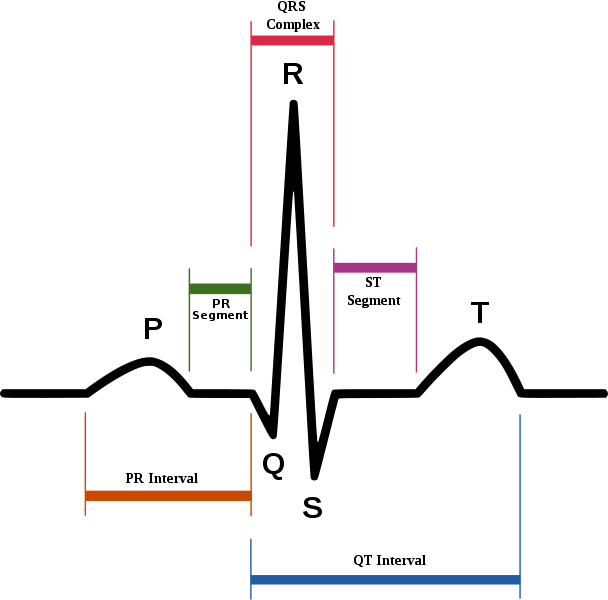
\includegraphics[scale=0.37]{./Abrak/Egyeb/ecg_wiki.png}
   \caption{Az EKG jel egy szívütése, illetve annak főbb diagnosztikai jellemzői.}
		\label{fig:ekg}
\end{center}
\end{figure}
 
Az irodalomban ismert tömörítő algoritmusokat \cite{unifiedReview} alapján három kategóriába sorolhatjuk: 1) egyszerű paraméteres becslések (pl.: interpoláció, különbségi kódolás, stb.), 2) direkt módszerek (pl.: csúcsok, meredekségek, stb. tárolása), 3) transzformációs eljárások. Az utóbbi osztály tartalmazza azokat az algoritmusokat, melyek a jelet egy előre adott függvényrendszer szerinti sorfejtéssel approximálják. Így az eredeti adatsorozat helyett csak az együtthatókat és a rendszer paramétereit kell tárolnunk. Ezen kategóriába sorolandó a dolgozatban bemutatott algoritmus is. Nevezetesen, az eredeti adatsorozatot speciális, Hermite-polinomok segítségével előállitott függvényrendszerrel fogjuk közelíti. A módszer alapját képező eljárás \cite{hexp3}, jól ismert az irodalomban, mely nem csak a jelek tömörítéséhez, de azok modellezéséhez \cite{hexp2}, illetve osztályozásához \cite{hexp1, hexp4} is alkalmazható. A dolgozatban az EKG jelekkel való hasonlóságuk miatt Hermite-függvényeket használunk az adatok reprezentálásához. Ezeket egy argumentum transzformáción keresztül szabad paraméterekkel egészítjük ki. Ennek köszönhetően az eredeti jelet egy adaptív bázisban írhatjuk fel. Az említett paraméterek megválasztásához a Nelder-Mead optimalizációs eljárást alkalmaztuk. Mivel az EKG jelek diszkrét adatsorozatok, ezért a módszert \cite{hexp5} alapján implementáltuk diszkrét ortogonális Hermite-polinomokra is. A dolgozatban különböző tesztekkel demonstráljuk az algoritmus hatékonyságát. Ehhez, több órányi, zajjal terhelt, valódi EKG felvételt használtunk. Ezen keresztül a bemutatott módszert összehasonlítottuk több másik, az irodalomban jól ismert tömörítő algoritmussal is \cite{jpeg2000ECG}. 

A tömörítő eljárást egy c++ nyelven megírt, objektum elvű alkalmazás implementálja, melyet egy webes felületen keresztül érhetünk el. A felület lehetőséget biztosít a dolgozatban jelölt tesztek újrafuttatására, valamint a teszteléskor felhasznált adatbázis további jeleinek a tömörítésére. Szintén a webes felületen keresztül nyílik alkamunk a már tömörített EKG jelek helyreállítására. 

Az alkalmazás megetrvezésekor külön hangsúlyt kapott a kód újra felhasználhatósága. Ennek érdekében a felhasznált algoritmusok, illetve matematikai modellek a lehető legáltalánosabb formában lettek implementálva. Fontos szempontot jelentett továbbá a c++11-es nyelvszabvány által nyújtotta lehetőségek minél hatékonyabb kihasználása. Jó példa erre a lambda függvények alkalmazása az optimalizációs algoritmusok implementációja során. A hatékony működés mellett azonban a program igyekszik megfelelni a modern felhasználók igényeinek. Ennek érdekében a felhaszálói felület weboldalként lett implementálva. A rendszerfüggetlen, és installáció mentes elérés lehetővé teszi a gyors és egyszerű használatot, valamint az eredmények megosztását.  

\section{Matematikai háttér}
\subsection{Jelek approximációja}

EKG jelek feldolgozásakor sok esetben szembesülünk gyakorlati kihívásokkal. Két sűrűn előforduló példa a hosszú mérések tárolása, valamint a zajjal terhelt mérések ábrázolása. Ezekre a nehézségekre egyszerre ad kielégítő megoldást, ha a jeleket  valamely $\mathcal H$ Hilbert-tér sima függvényeiből álló $(\Phi_n, n\in\Bbb N)$ ortogonális bázisában reprezentáljuk és a jelet véges sok $\Phi_0,\Phi_1,\cdots,\Phi_n$ bázisbeli elem lineáris kombinációjával közelítjük. Az $f\in\mathcal H$ jel
legjobb közelítését a tér $\|\cdot\|$ normájában az
$$
S_nf:=\sum_{k=0}^n\langle f,\Phi_k\rangle \Phi_k
$$
leképezés nyújtja, ahol $\langle\cdot,\cdot\rangle$ az $\mathcal  H$ tér
skaláris szorzatát jelöli. A jel és a közelítés eltérésének négyzete  a
$$
\|f-S_nf\|^2=\|f\|^2-\sum_{k=0}^n|\langle f,\Phi_k\rangle|^2
$$
képplettel adható meg. Adott hibán belüli közelítést véve a jel helyett  elég az
$S_nf$ approximációt reprezentáló  $\langle f,\Phi_k\rangle\ (k=0,1,\cdots, n)$ Fourier-együtthatókat tárolni.  Zajos jel esetén az ilyen típusú approximáció szűrőként is szolgál.  A közelítés megvalósításához a klasszikus ortogonális rendszerek közül  EKG görbék közelítésére  az Hermite-féle függvények bizonyultak használhatónak. Ezt támasztják alá a [...] dolgozatok. Az  Hermite függvények alkalmazása azzal is indikolható, hogy grafikonjuk hasonlí t az EKG görbékre (lásd a Függeléket).



\section{Az approximáció optimalizálása}

\chapter{Felhasználói dokumentáció}

\chapter{Fejlesztői dokumentáció}

\end{document}
